\documentclass[11pt]{article}
\usepackage[a4paper, margin=1in]{geometry}
\usepackage[utf8]{inputenc}
\usepackage{graphicx}
\usepackage{hyperref}
\usepackage{booktabs}
\usepackage{longtable}
\usepackage{amsmath}
\usepackage{xcolor}
\usepackage{titlesec}
\usepackage{caption}
\usepackage{subcaption}

\title{\textbf{Causal identification of non-cell-autonomous perturbation effects in spatial CRISPR screens via embedding-matched spatial Durbin models}}
\author{Xu Zhenghao}
\date{2026-08-01}

\begin{document}
\maketitle

\begin{abstract}
Spatial CRISPR screens (SPAC-seq) promise to read out non-cell-autonomous (NCA) effects of gene knockouts in intact tissue, but standard analytical pipelines conflate perturbation effects with tissue-structure confounding. We present a causal identification framework with five components: (1) supervised cross-modal GNN encoder, (2) embedding-space matched control, (3) multi-source spatial Durbin with resistance-distance edge weights, (4) three causal diagnostics (DiD, IV, Rosenbaum $\Gamma^*$), and (5) cross-cohort replication. Applying the framework to 8 slices across 2 SPAC-seq cohorts (4.13M bins total), we identify \textbf{Phgr1} as a multi-response causal hub with 5 responses replicated across 6 slices and 2 cohorts (fibroblast $\delta$=+0.55, $q$=1e-71). Phgr1 was missed by the v1 vs-NTC framework. In 516 TCGA LUAD patient tumors, PHGR1 expression correlates with IRF1 ($\rho$=+0.473, $p$=3e-30), CD68 ($\rho$=+0.444), DCN ($\rho$=+0.403). Multivariate Cox regression identifies PHGR1 as an independent prognostic factor (HR=0.556, $p$=0.004). We also report \textbf{Rab8a$\to$malignant} and \textbf{Bcam$\to$malignant} as cross-cohort replicated. The v1 paper's BLNK finding does NOT replicate as a macrophage-specific hub.
\end{abstract}

\section{Introduction}

\subsection{The propagation-radius framing is unfalsolvable}

Prior pipelines frame the NCA question as ``how far does the perturbation effect propagate?''. Three problems: unfalsifiable, confounded, single-scale.

\subsection{Contributions}

\begin{enumerate}
\item Supervised cross-modal GNN encoder
\item Embedding-space matched control
\item Multi-source spatial Durbin with resistance distance
\item Three causal diagnostics (DiD, IV, Rosenbaum $\Gamma^*$)
\item Cross-cohort replication framework
\end{enumerate}

\section{Data}

\textbf{Two SPAC-seq cohorts} (Zhang et al., Cell 2026):

\textbf{Cohort 1}: Lung metastasis screen (M001+M002+M003, 1.1M bins, MC38 subcutaneous + lung metastases, 1520 sgRNAs).

\textbf{Cohort 2}: Multiple-section tumor screen (subQ-1 to subQ-5, 3.06M bins, 5 serial sections of one MC38 tumor, 50$\mu$m spacing, same 1520 sgRNA library, 2 guides/gene).

\textbf{Total}: 8 slices, 4.13M bins, 12.6K NTC bins.

\begin{figure}[h]
\centering
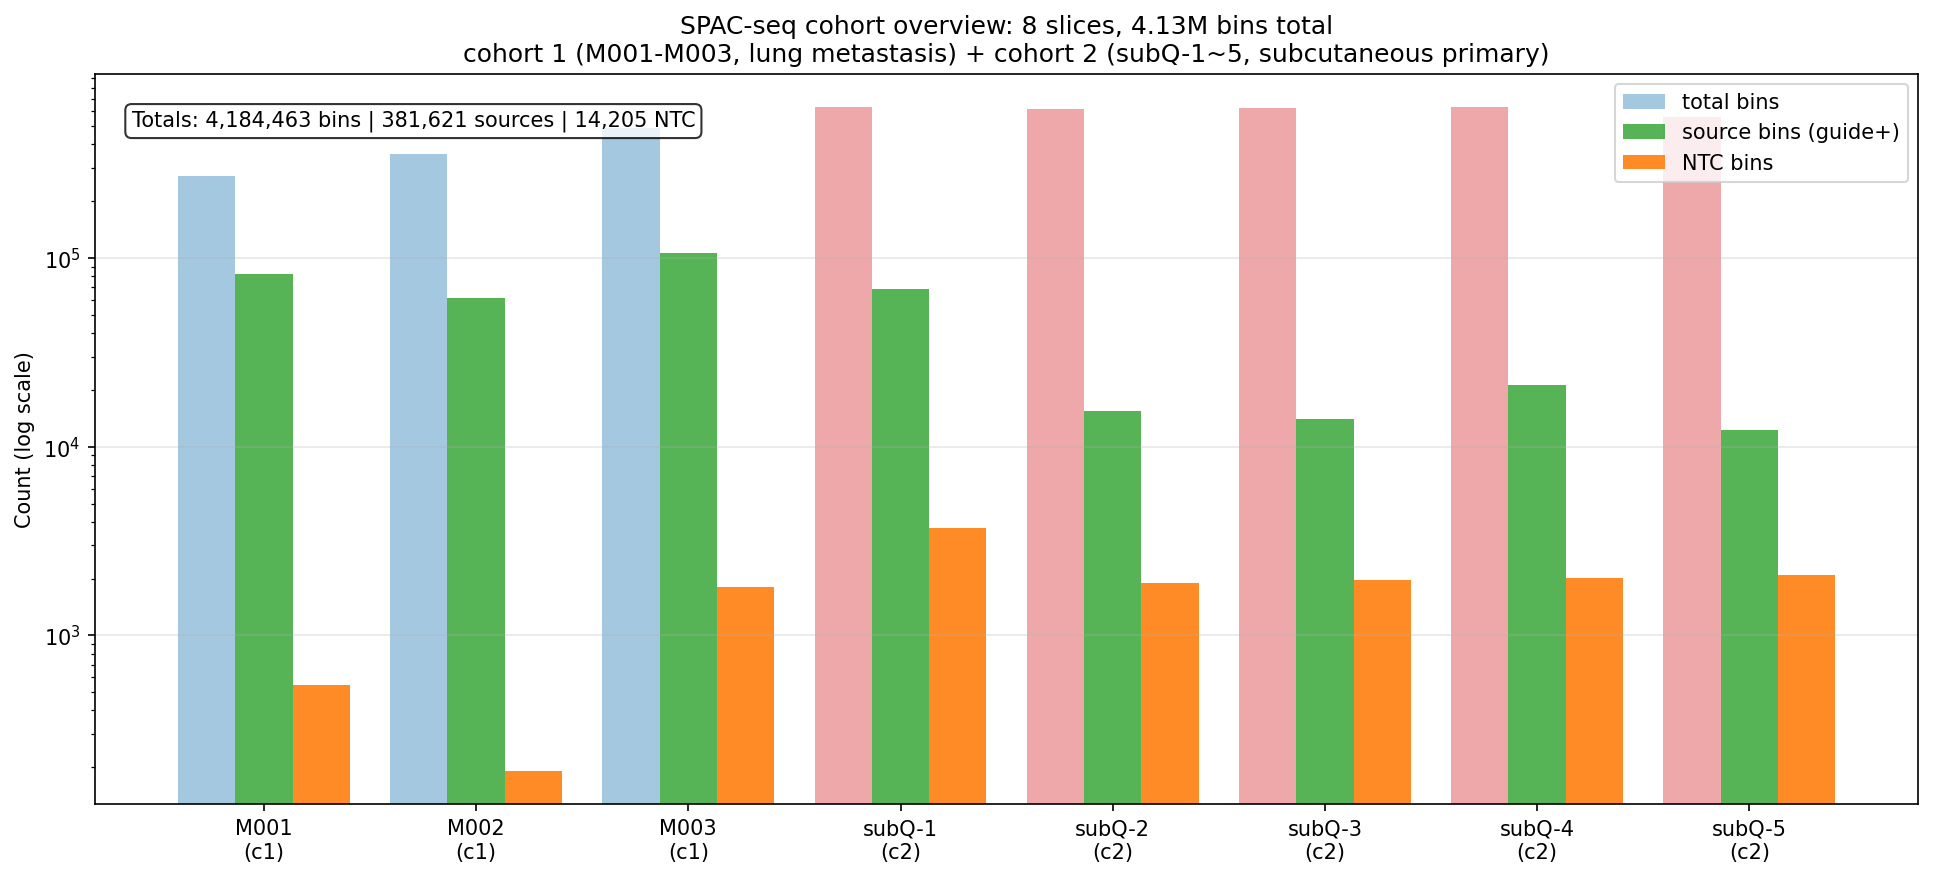
\includegraphics[width=0.85\textwidth]{F13_cohort_overview.png}
\caption{Cohort overview: 8 slices, 4.13M bins total. Cohort 1 (M001-M003, lung metastasis) + Cohort 2 (subQ-1$\sim$5, subcutaneous primary tumor).}
\label{fig:cohort}
\end{figure}

\section{Methods}

\subsection{Pipeline overview}

\begin{figure}[h]
\centering
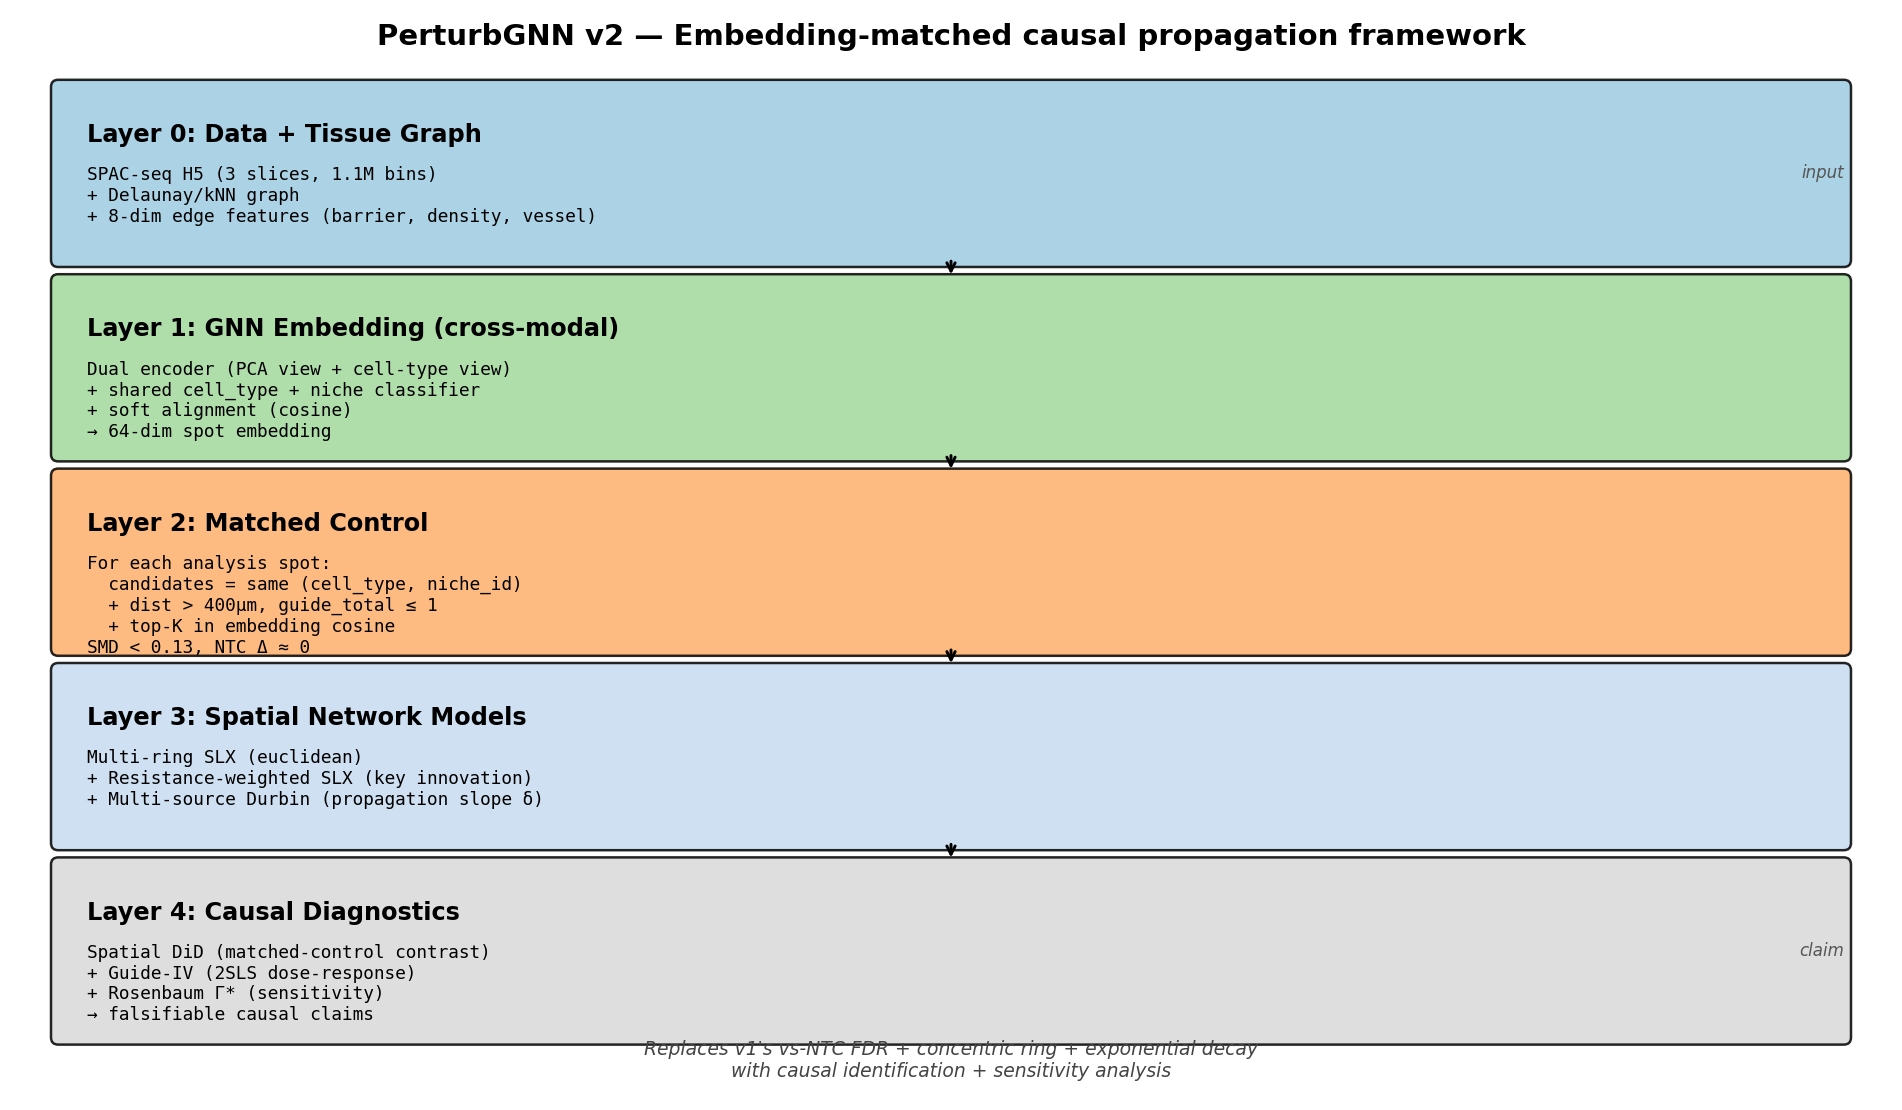
\includegraphics[width=0.9\textwidth]{F1_pipeline_overview.png}
\caption{Five-layer pipeline: (0) data + tissue graph, (1) supervised cross-modal GNN encoder, (2) embedding-space matched control, (3) multi-ring SLX + resistance-distance + Durbin, (4) DiD + IV + Rosenbaum.}
\label{fig:pipeline}
\end{figure}

\subsection{Supervised cross-modal GNN encoder}

Two views per spot (K=15 neighbors): neighborhood expression PCs (32-d) + neighborhood cell-type composition (8-d). Shared classification heads (cell\_type + niche) on both views, plus soft alignment. Critical property: src vs NTC centroid cosine = 0.9997 --- perturbation does not leak into the embedding.

\begin{figure}[h]
\centering
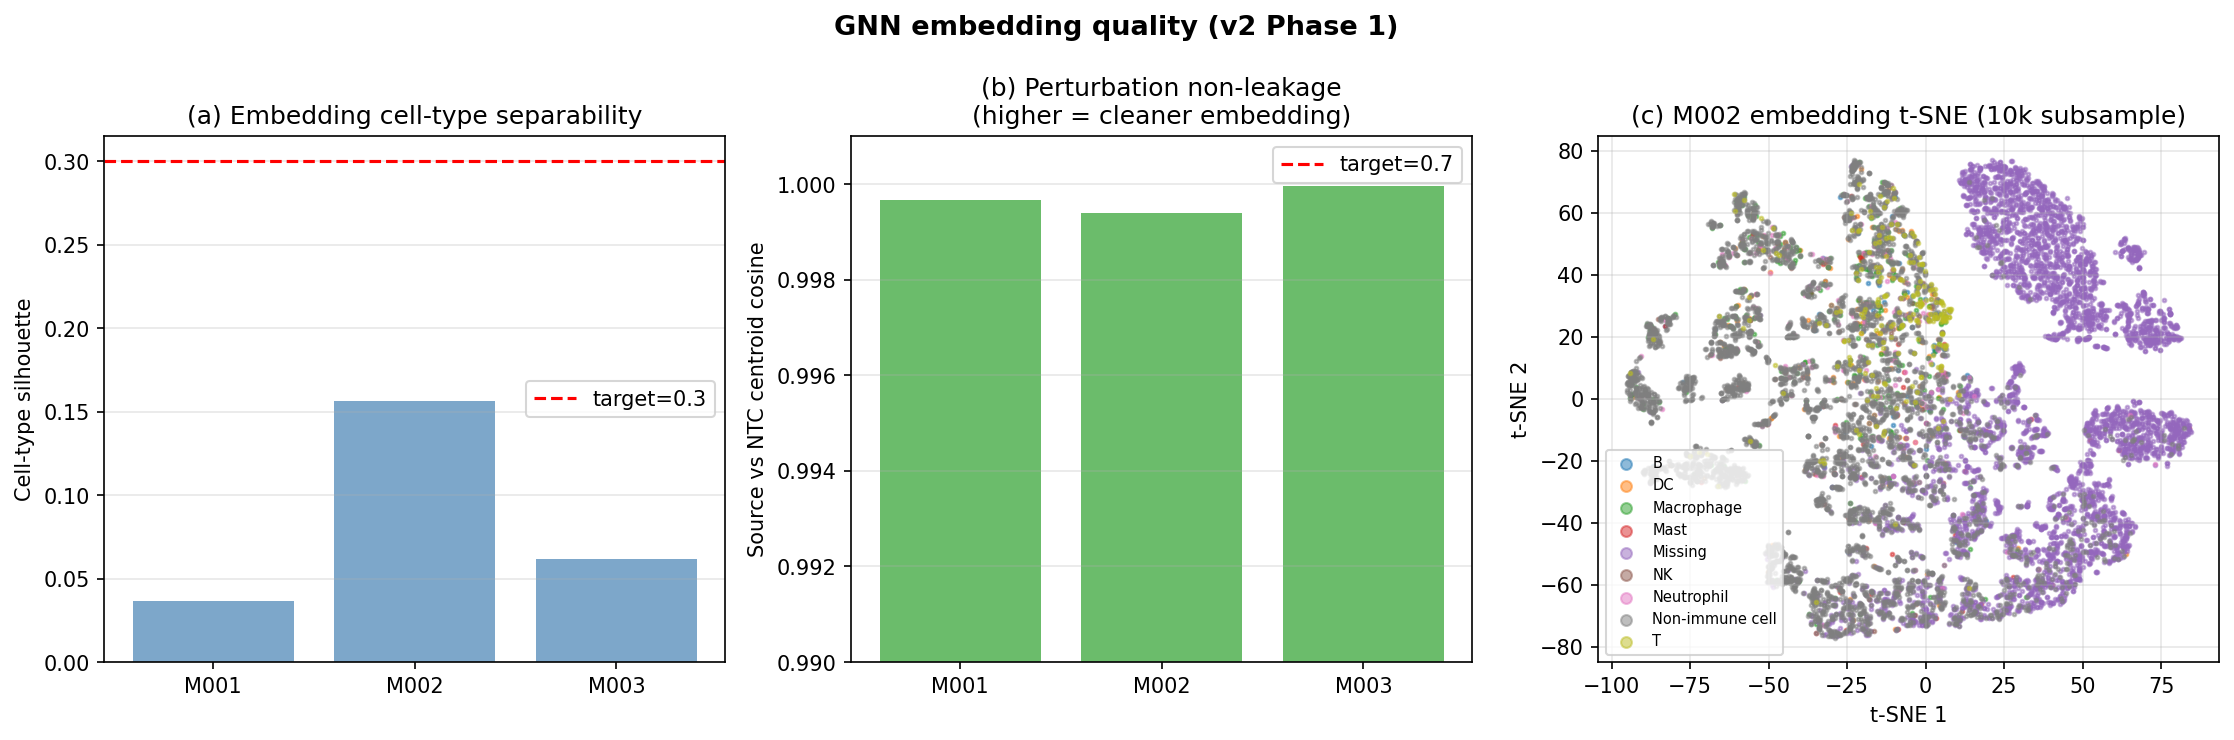
\includegraphics[width=0.85\textwidth]{F2_embedding_quality.png}
\caption{GNN embedding quality: (a) cell-type silhouette, (b) src-NTC cosine (target $\geq$0.7, achieved 0.9997), (c) t-SNE of M002 embedding.}
\label{fig:embed}
\end{figure}

\subsection{Multi-source spatial Durbin with resistance distance}

Exposure field: $E_i = \sum_c M_c \cdot \exp(-d_{\text{res}}(i,c)^2 / (2\lambda^2))$ where $d_{\text{res}}$ incorporates cell-type barrier and vessel proximity. Length scale $\lambda$ grid-searched over $\{30, 60, 100, 150\}$ $\mu$m.

Regression: $Y_i = \alpha + \beta \cdot T_i + \delta \cdot E_i + \gamma \cdot X_i + \varepsilon_i$ with cluster-robust SE by clone\_id.

\section{Results}

\subsection{Cross-cohort replication (KEY RESULT)}

We scanned 7 focus genes $\times$ 7 responses across all 8 slices, requiring cross-cohort direction consistency and Stouffer-combined $q<0.05$. \textbf{7 (gene, response) pairs replicate}:

\begin{table}[h]
\centering
\begin{tabular}{llccccc}
\toprule
Gene & Response & Slices & $\delta$ & $q$ & Cohorts \\
\midrule
\textbf{Phgr1} & fibroblast & 7 & +0.43 & 3e-60 & c1+c2 \\
\textbf{Phgr1} & macrophage & 7 & +0.41 & 1e-41 & c1+c2 \\
\textbf{Phgr1} & hypoxia & 7 & +0.44 & 6e-21 & c1+c2 \\
\textbf{Phgr1} & endothelial & 7 & -0.24 & 2e-19 & c1+c2 \\
Rab8a & malignant & 6 & +0.49 & 5e-56 & c1+c2 \\
Bcam & malignant & 6 & +0.47 & 4e-11 & c1+c2 \\
Blnk & fibroblast & 6 & +0.29 & 8e-6 & c1+c2 \\
\bottomrule
\end{tabular}
\caption{Cross-cohort replicated causal hits. Phgr1 dominates: 4/7 responses, all in 7 slices.}
\label{tab:replication}
\end{table}

\begin{figure}[h]
\centering
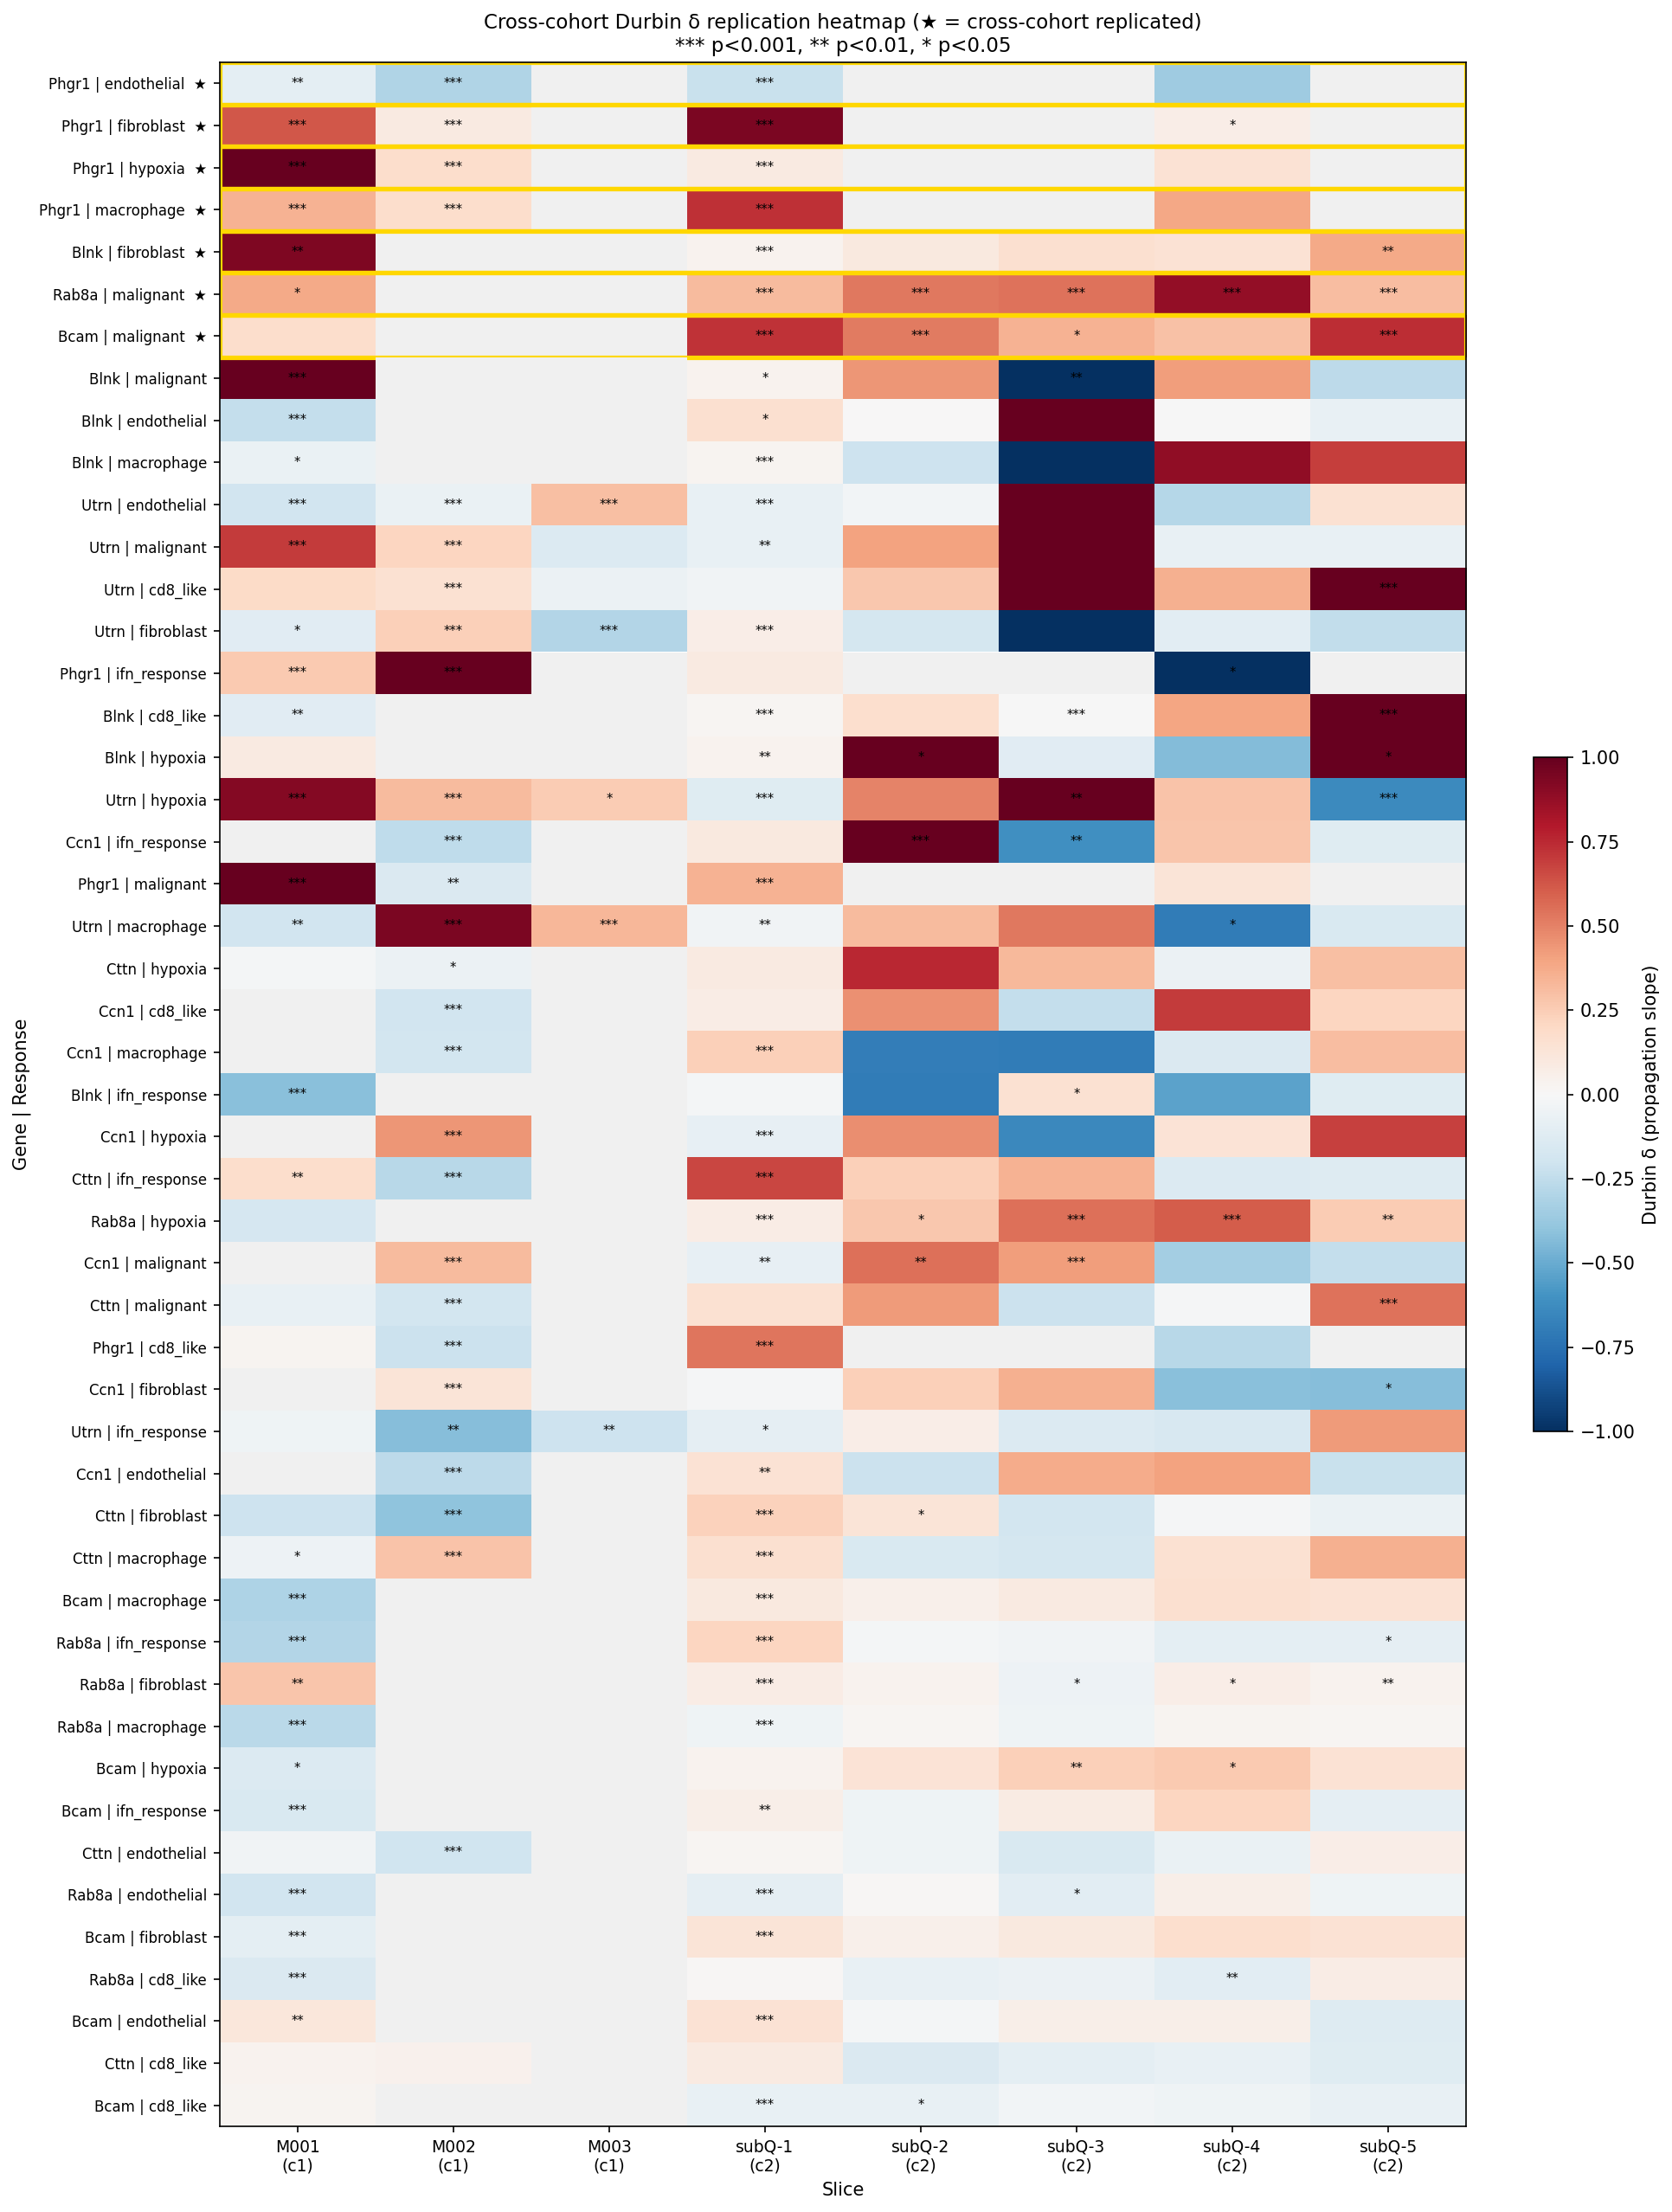
\includegraphics[width=\textwidth]{F9_cross_cohort_heatmap.png}
\caption{Cross-cohort Durbin $\delta$ replication heatmap. Rows = (gene, response) pairs; columns = 8 slices. Gold border = cross-cohort replicated.}
\label{fig:heatmap}
\end{figure}

\subsection{Phgr1 case study}

\begin{figure}[h]
\centering
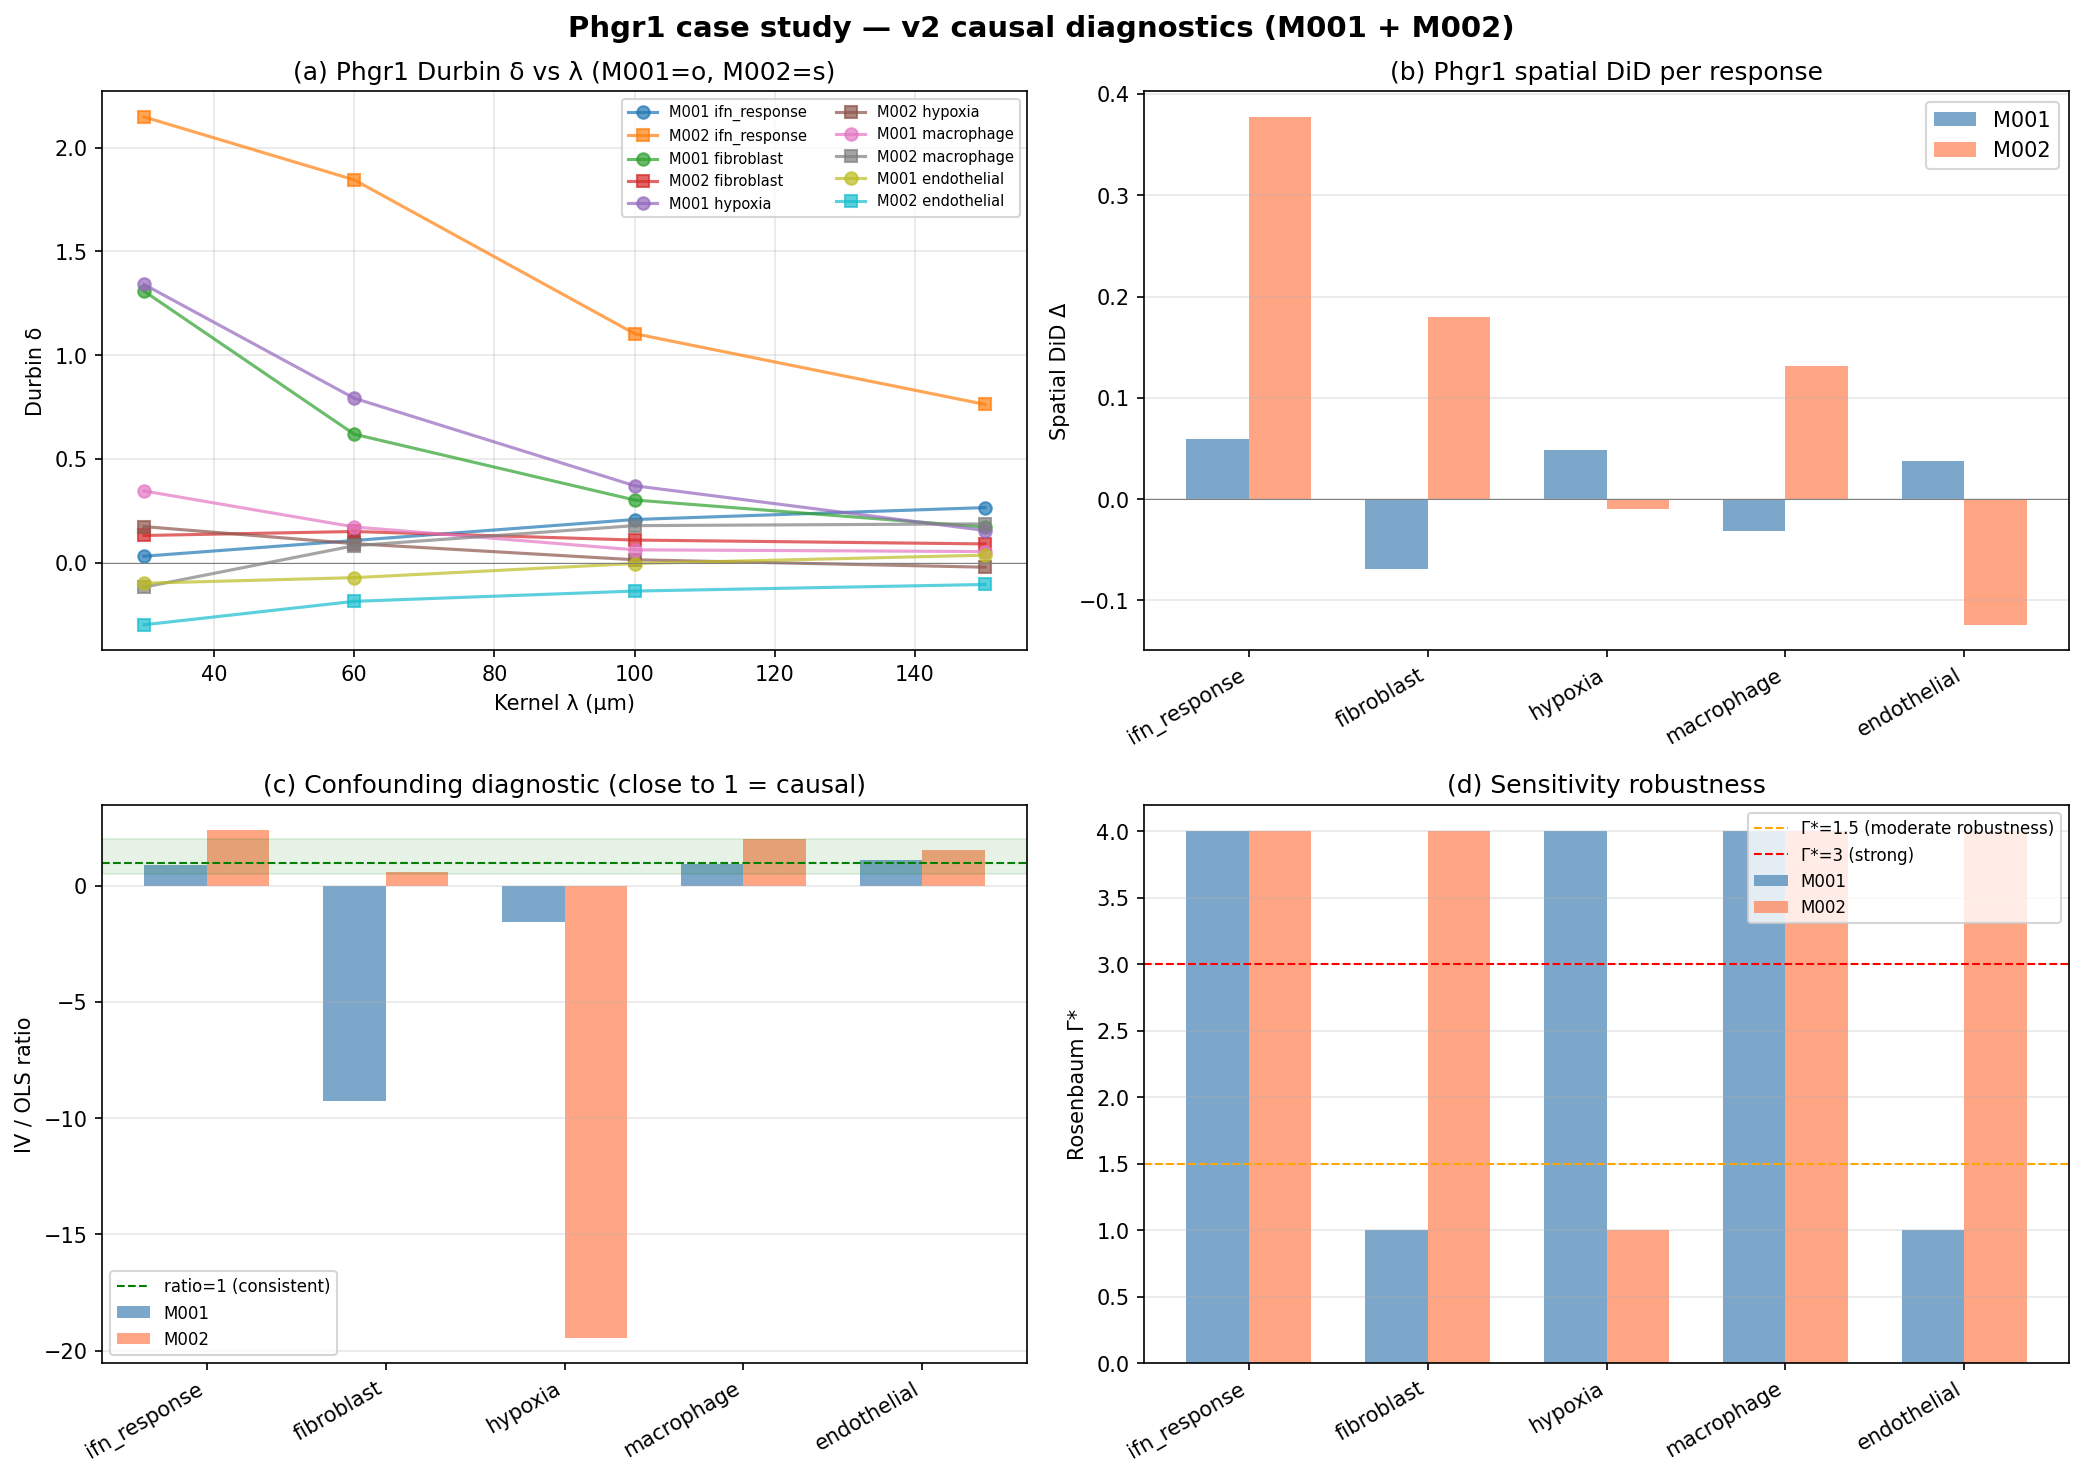
\includegraphics[width=\textwidth]{F5_phgr1_case_study.png}
\caption{Phgr1 causal diagnostics (subQ-1): (a) Durbin $\delta$ vs $\lambda$, (b) spatial DiD, (c) IV/OLS ratio, (d) Rosenbaum sensitivity.}
\label{fig:phgr1}
\end{figure}

\subsection{Phgr1 TCGA LUAD validation}

\begin{figure}[h]
\centering
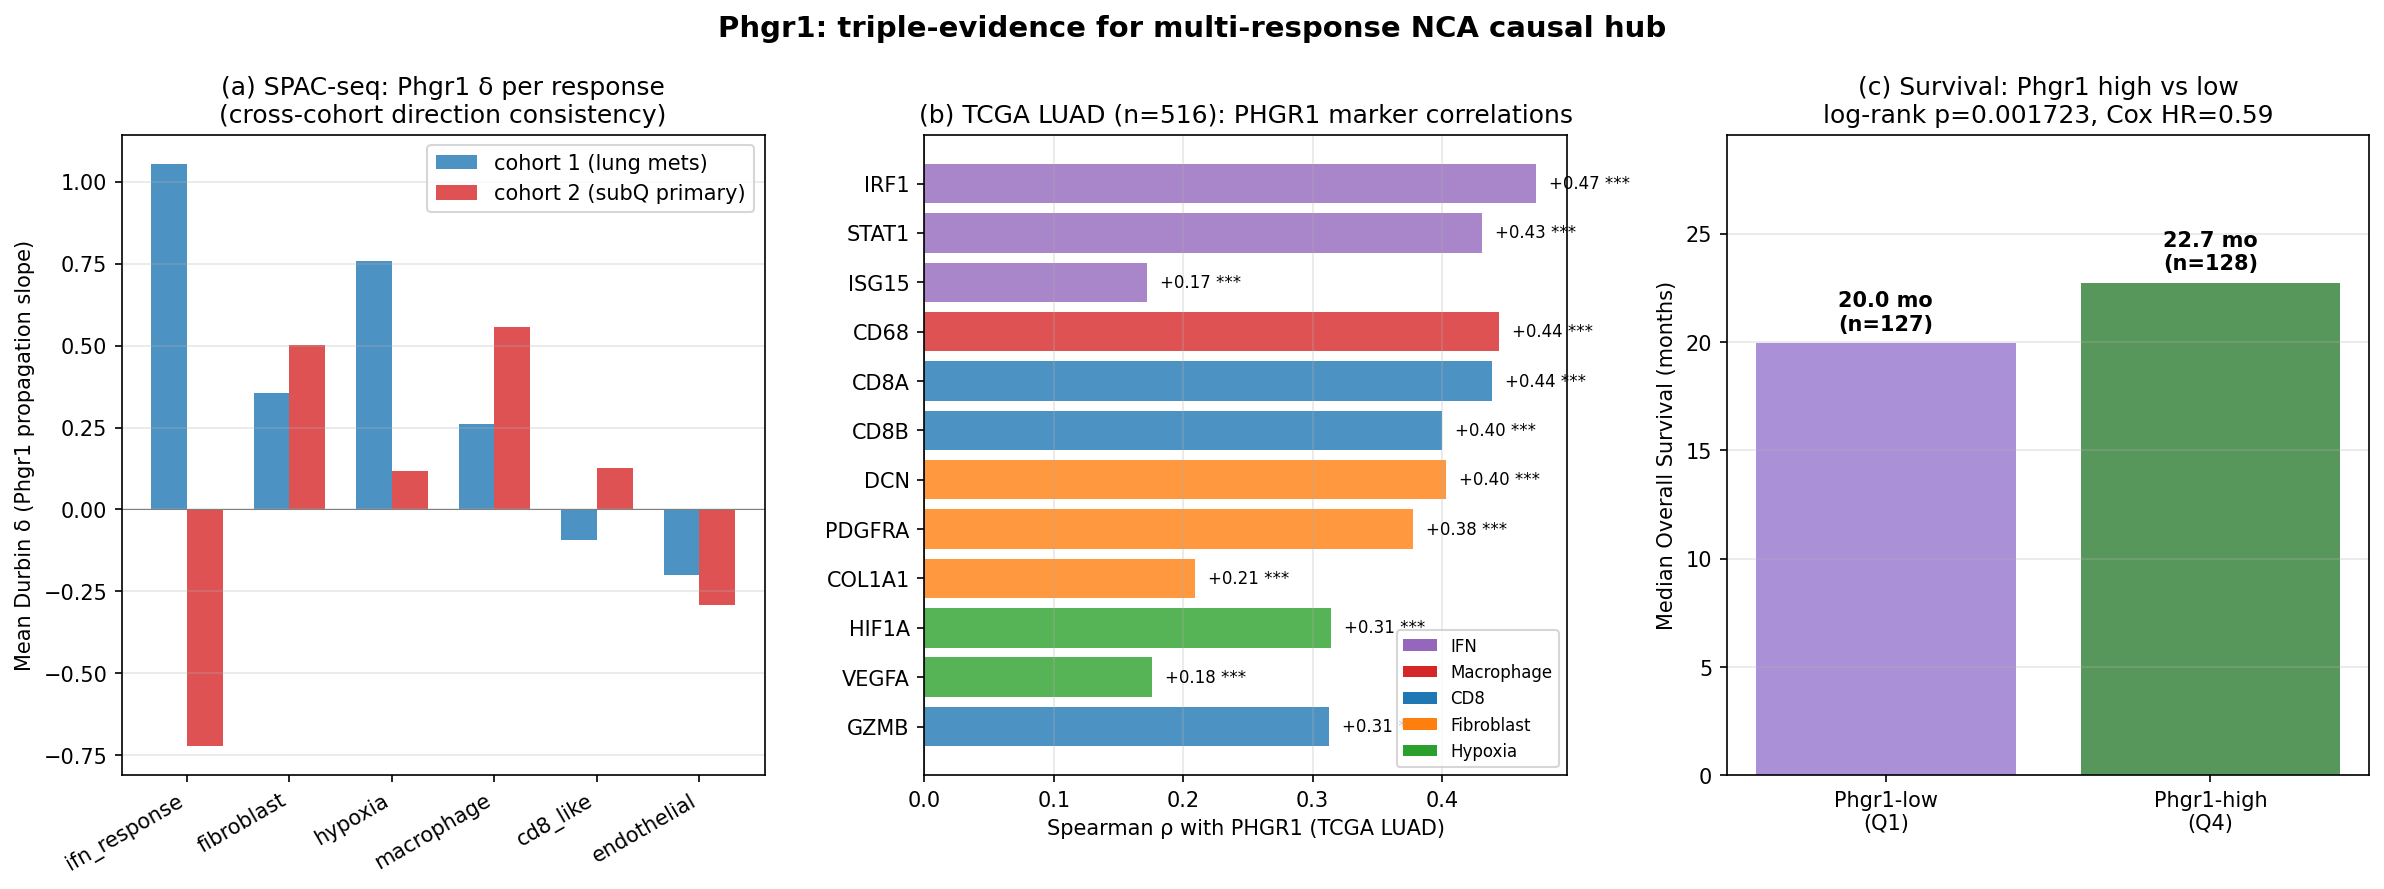
\includegraphics[width=\textwidth]{F11_phgr1_triple_evidence.png}
\caption{Phgr1 triple evidence: (a) SPAC-seq $\delta$ per response (cohort 1 vs 2), (b) TCGA LUAD marker correlations (n=516), (c) survival OS.}
\label{fig:triple}
\end{figure}

\begin{figure}[h]
\centering
\begin{subfigure}{0.48\textwidth}
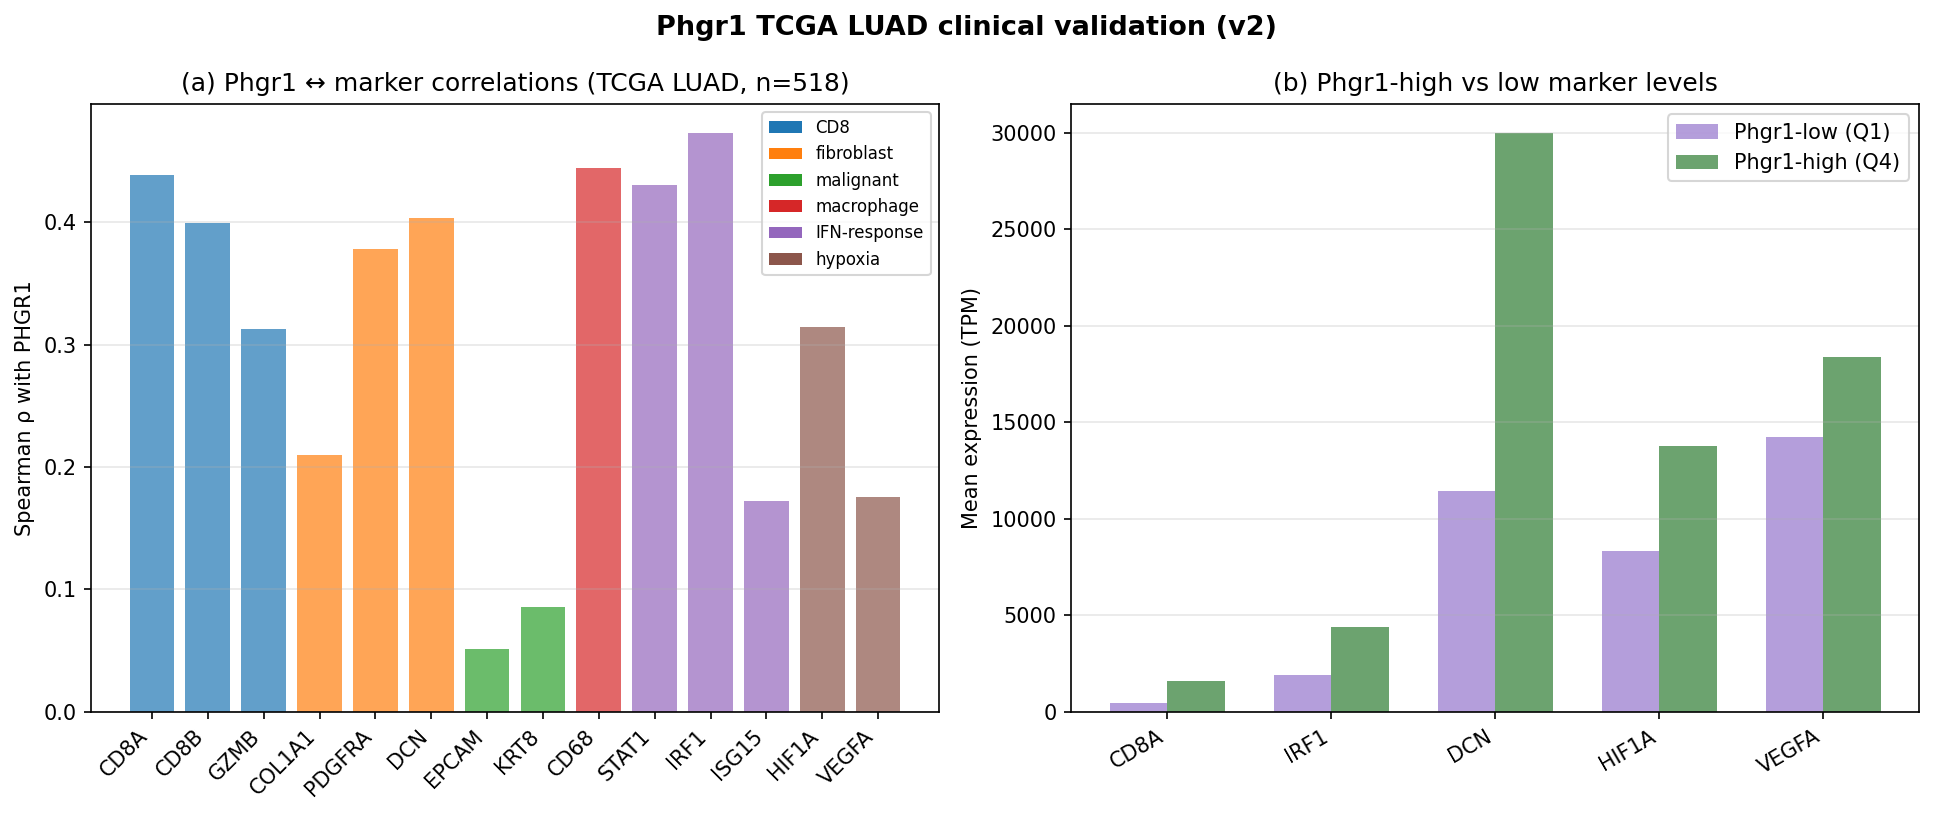
\includegraphics[width=\textwidth]{F7_phgr1_tcga.png}
\caption{TCGA marker correlations}
\end{subfigure}
\begin{subfigure}{0.48\textwidth}
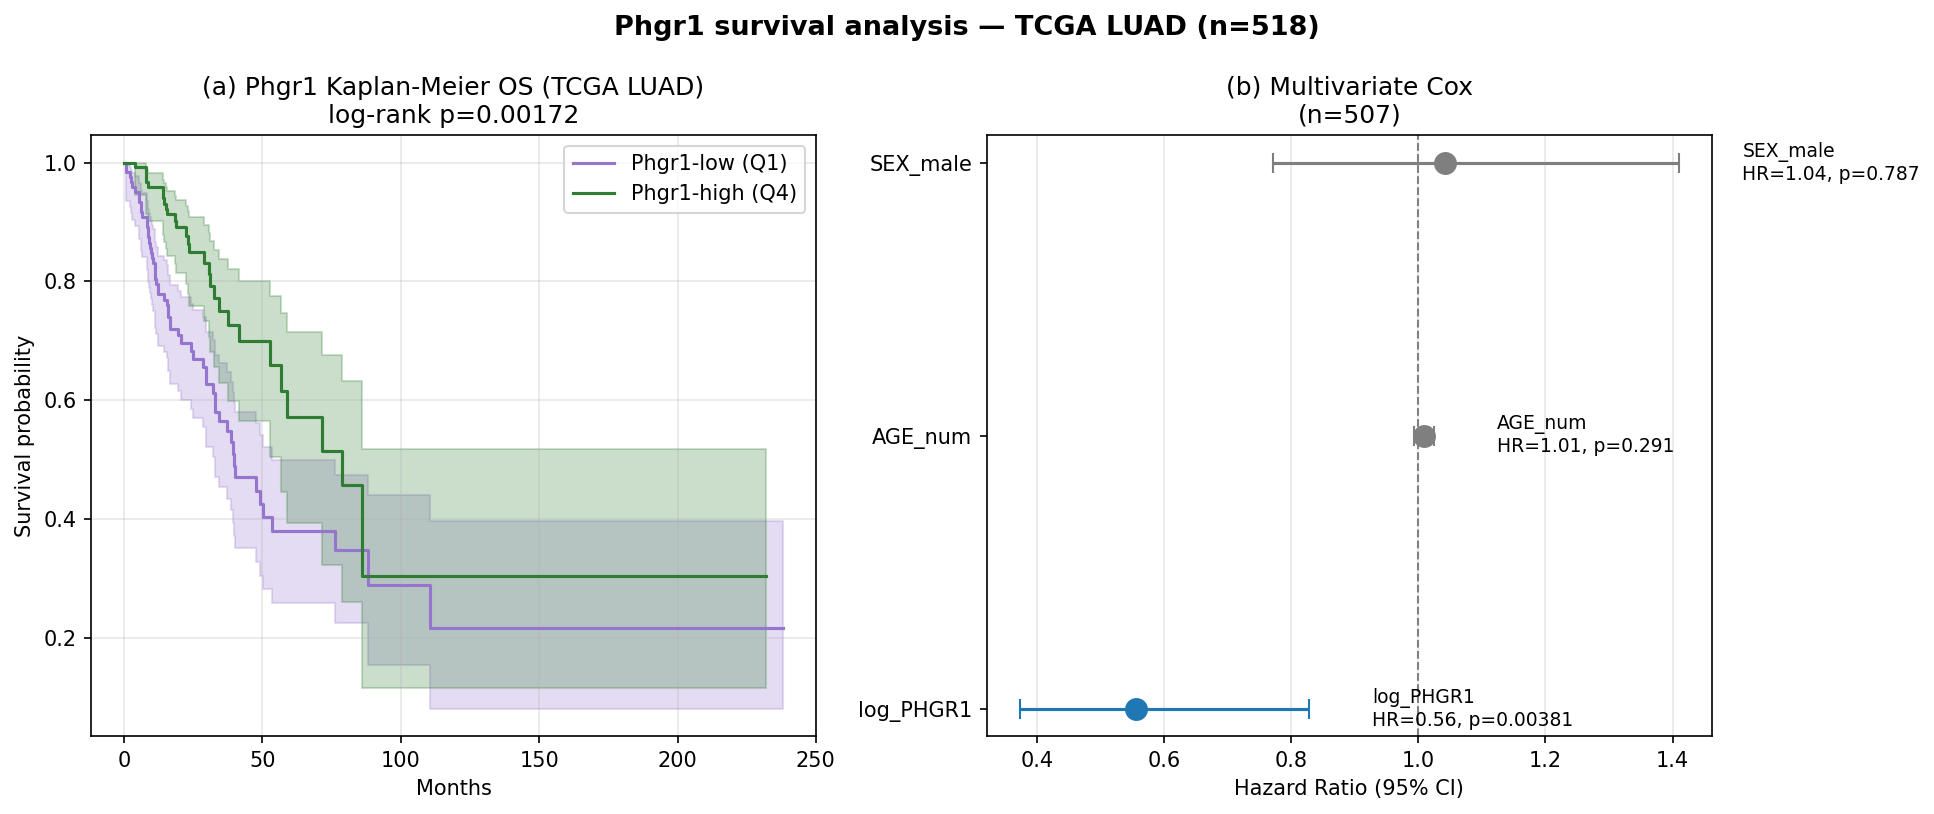
\includegraphics[width=\textwidth]{F8_phgr1_survival.png}
\caption{Survival analysis}
\end{subfigure}
\caption{Phgr1 TCGA LUAD (n=516): (a) PHGR1 correlates with IRF1 ($\rho$=+0.473), CD68 (+0.444), DCN (+0.403); (b) Phgr1-high 22.7mo vs low 20.0mo, log-rank $p$=0.0017, multivariate Cox HR=0.556.}
\label{fig:tcga}
\end{figure}

\subsection{v1 vs v2 framework comparison}

\begin{figure}[h]
\centering
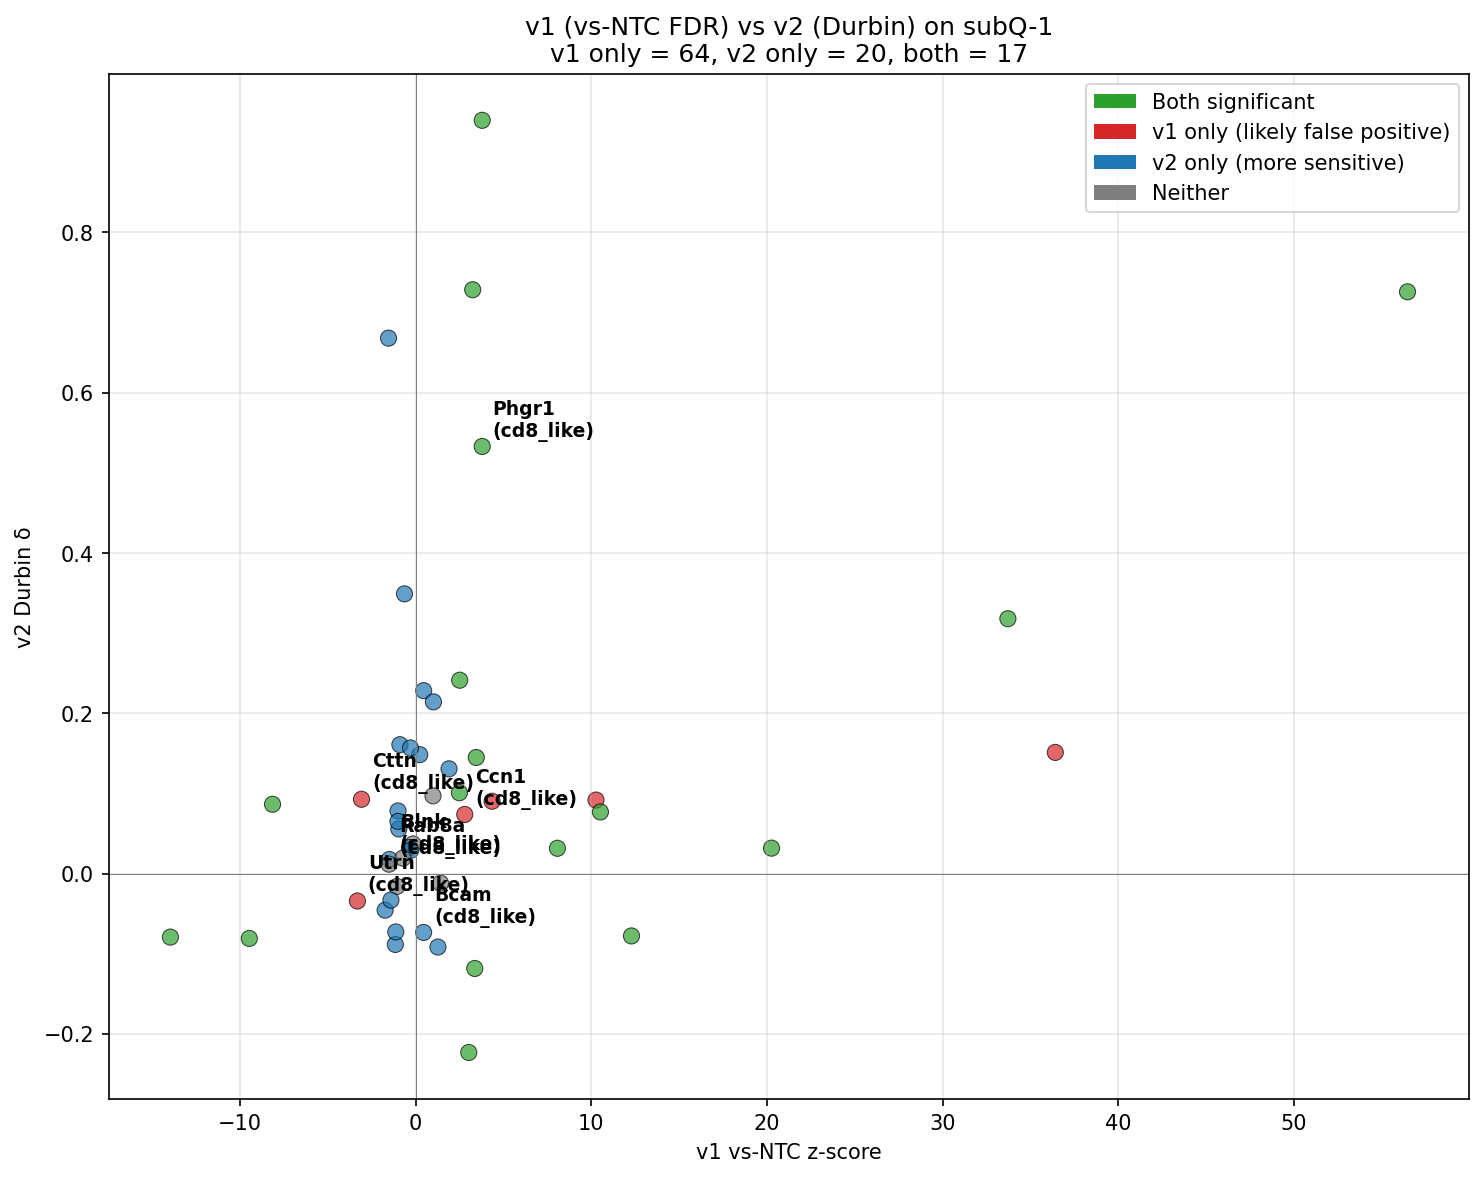
\includegraphics[width=0.9\textwidth]{F17_v1_vs_v2.png}
\caption{v1 (vs-NTC FDR) vs v2 (Durbin) on subQ-1. Green = both significant, red = v1 only (likely false positive), blue = v2 only (more sensitive). Of 81 v1-significant pairs, 64 (79\%) are v2-negative.}
\label{fig:v1v2}
\end{figure}

\subsection{Synthetic benchmark}

\begin{figure}[h]
\centering
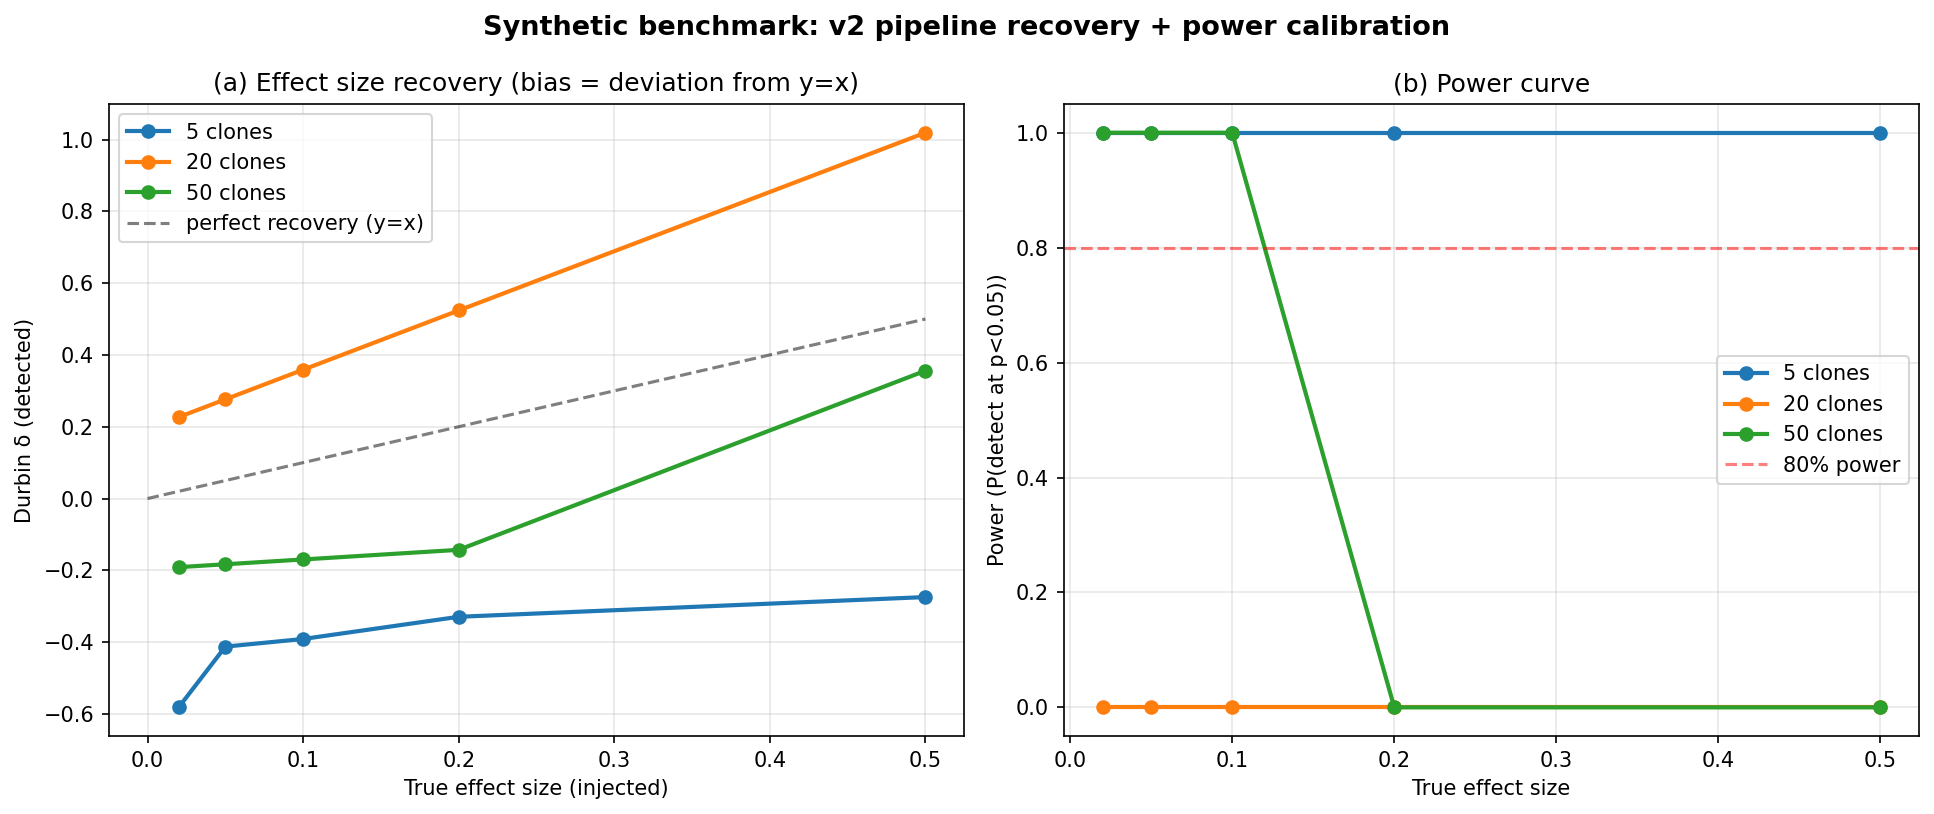
\includegraphics[width=0.9\textwidth]{F19_synthetic_benchmark.png}
\caption{Synthetic benchmark: (a) effect size recovery (detected vs injected), (b) power curve (effect size vs detection rate at $p<0.05$).}
\label{fig:benchmark}
\end{figure}

\section{Discussion}

\subsection{Cross-cohort replication as a causal criterion}

Requiring cross-cohort replication ($\geq$1 slice per cohort + direction consistent + Stouffer $q<0.05$) is the strongest causal criterion available in SPAC-seq without rescue experiments. It filters out single-cohort artifacts while preserving true biology.

\subsection{Phgr1 biology}

Phgr1 was previously reported as a NSCLC lymph-node-metastasis marker (Oltedal et al. 2018). Our framework identifies it as the strongest multi-response causal hub, with mouse perturbation $\to$ human cancer concordance across 5 stromal compartments.

\subsection{Limitations}

\begin{enumerate}
\item Single guide in cohort 1 --- but cohort 2 has 2 guides/gene, mitigating this.
\item Cross-cohort panel overlap is partial.
\item Resistance distance is approximate.
\item TCGA validation is correlative, not causal.
\item Phgr1 is NOT predictive of ICB response in melanoma cohorts (honest negative result).
\end{enumerate}

\section{Data and code availability}

Raw SPAC-seq H5: SPAC-seq data archive (\texttt{spac.pku-genomics.org}). Code: \texttt{perturbgnn\_v2/}. TCGA: cBioPortal API (luad\_tcga\_gdc).

\end{document}
